\def\year{2021}\relax
\documentclass{article}
\pdfpagewidth=8.5in
\pdfpageheight=11in
% The file ijcai21.sty is NOT the same than previous years'
\usepackage{ijcai21}

% Use the postscript times font!
\usepackage{times}
\usepackage{soul}
\usepackage{url}
\usepackage[hidelinks]{hyperref}
\usepackage[utf8]{inputenc}
\usepackage[small]{caption}
\usepackage{graphicx}
\usepackage{helvet}
\usepackage{amsthm}
\usepackage{booktabs}
\usepackage{algorithm}
\usepackage{algorithmic}
\usepackage{subcaption}
\urlstyle{same}


\usepackage{amsmath, amssymb}
\usepackage{subcaption}
\usepackage[dvipsnames]{xcolor}
\usepackage{latexsym}
\newcommand{\ra}[1]{\renewcommand{\arraystretch}{#1}}
\newtheorem{theorem}{Theorem}
\newtheorem{proposition}{Proposition}
\newtheorem{conjecture}{Conjecture}
\newtheorem{definition}{Definition}
\frenchspacing
\newtheorem{lemma}{Lemma}
\DeclareMathOperator*{\argmin}{arg\,min}
\DeclareMathOperator*{\argmax}{arg\,max}
\def\tuple#1{( #1 )}

\setcounter{secnumdepth}{2}
\pdfinfo{
/Author (Naftali Waxman,
Sarit Kraus, Noam Hazon)
/TemplateVersion (IJCAI.2021.0)
}

\title{Manipulation of k-Coalitional Games on Social Networks }
\author{%Paper \#4621

    %Authors
    % All authors must be in the same font size and format.
    Naftali Waxman$^1$
    \and
    Sarit Kraus$^1$
    \And
     Noam Hazon$^2$
     \affiliations
    $^1$Bar-Ilan University, Israel\\
    $^2$Ariel University, Israel\\
    \emails
    \{sarit, vaxmann\}@cs.biu.ac.il,
    noamh@ariel.ac.il
}



%
\begin{document}
\maketitle
\begin{abstract}
In many coalition formation games the utility of the agents depends on a social network. In such scenarios there might be a manipulative agent that would like to manipulate his connections in the social network in order to increase his utility. We study a model of coalition formation in which a central organizer, who needs to form k coalitions, obtains information about the social network from the agents.
The central organizer has her own objective: she might want to maximize the utilitarian social welfare, maximize the egalitarian social welfare, or simply guarantee that every agent will have at least one connection within her coalition. 
In this paper we study the susceptibility to manipulation of these objectives, given the abilities and information that the manipulator has. Specifically, we show that if the manipulator has very limited information, namely he is only familiar with his immediate neighbours in the network, then a manipulation is almost always impossible. Moreover, if the manipulator is only able to add connections to the social network, then a manipulation is still impossible for some objectives, even if the manipulator has full information on the structure of the network. On the other hand,  if the manipulator is able to hide some of his connections, then all objectives are susceptible to manipulation, even if the manipulator has limited information, i.e., when he is familiar with his immediate neighbours and with their neighbours.


\end{abstract}
%We study a model of coalition formation where exactly $k$ coalitions must be formed and the agents' utility depends on a social network. A central organizer who forms the coalitions obtains information about the social network from the agents.  In this context, we study the problem of an agent that would like to manipulate her connections in the network in order to increase her own utility. We study three main objectives for the organizer; maximizing the utilitarian social welfare, maximizing the egalitarian social welfare, and guaranteeing at least 1 neighbour for all of the agents. We analyze manipulator which has full information regarding the social network and one whose knowledge is limited to the network in her close proximity. We show that if  is able to hide some of her connections then all objectives are susceptible to manipulation. That is even when the manipulator is given limited knowledge, only about her neighbours and their neighbours. On the other hand, if the manipulator is only able to add connections, there are objectives for which manipulation is impossible, even if the manipulator is given full information. When the manipulator's knowledge is limited to her immediate neighbours only, almost always manipulation is impossible.

\section{Introduction}
% coalition formation in general
% cases with k-coalitional formation where organizer obtains information - example from high-school
% it is similar to voting where votere report 
% manipulatrion is voting is extensvely studied
% in our case- there is manipulation, but it has not studid
% we consider two types of manipulation - add or remove
% we consider 3 main objectives 
% ....
% table
%Hedonic games have been widely researched in the literature \cite{aziz2016computational}, and in particular ASHGs \cite{bogomolnaia2002stability}, from strategic point of view with emphasis on stable outcomes such as Nash equilibrium and the core \cite{aziz2011stable, peters2016graphical}. 
%The computational complexity of these problems have been studied in [ref]
%Hedonic games have also been studied from an optimization point of view, where the goal is to find a coalition formation maximizing a global utility function \cite{bachrach2013optimal, bansal2004correlation,charikar2005clustering}
Coalition formation is one of the fundamental research problems in multi-agent systems \cite{chalkiadakis2011computational}. 
Broadly speaking, coalition formation is concerned with partitioning a population of agents into disjointed teams (or coalitions) with the aim that some system-wide performance measure is maximized. Indeed, in many coalition formation games there is a central organizer that would like to maximize some objective.

%One assumption made in most coalition formation games is that any number of coalitions can be formed. In practice, in many real-world problems this assumption may not be true. For example, when dividing students into classes there is a known number of classes that have to be formed, and this number cannot be modified. There is no way to form more or less classes than agreed upon by the school and the administration. Another example is of assigning agents to complete tasks for a given project. If the project consists of $k$ tasks, any coalition structure with less than $k$ coalitions will not complete the project, and any coalition structure with more than $k$ coalitions includes redundant activity.
\begin{table*}[t]
\centering
\ra{1}
\begin{tabular}{@{}lcccc@{}}\toprule& \multicolumn{2}{c}{$Directed$} &  \multicolumn{2}{c}{$Undirected$}\\
\cmidrule{2-3} \cmidrule{4-5}
 & $Add$ & $Remove$ & $Add$ & $Remove$\\\midrule
\textbf{Max-Util} &
Strict(F~\ref{fig:Util_add}) & Strict(F~\ref{fig:Util_dir_remove}) & Strict(F~\ref{fig:Util_add})& Strict(F~\ref{fig:Util_remove_Improve})*\\
\textbf{Max-Egal} &
Strategyproof(T~\ref{thrm:egal_dir_add})& Strict(F~\ref{fig:Egal_directed_remove}) & LB,UB(F~\ref{fig:Egal_undirected_add_LB},\ref{fig:Egal_undirected_add_UB}), W-proof(T~\ref{thrm:egal_undir_add}) & Strict(F~\ref{fig:Egal_undirected_remove})\\
\textbf{At-least-1} &
Strategyproof(T~\ref{thrm:least1_add_dir}) & LB(F~\ref{fig:least1_remove}), UB-Proof(T~\ref{thrm:least1_remove}) & Strict(F~\ref{fig:Least1_undirected_add})& LB(F~\ref{fig:least1_remove}),UB-proof(T~\ref{thrm:least1_remove})\\
\bottomrule
\end{tabular}
\caption{Summary of the results.
The parentheses near a result refer to the corresponding figure (F) or theorem (T). The results hold for both full information and distance 2, except for the result with the * , which holds only for the full information case. Key: LB/UB/Strict = the objective is subject to LB/UB/Strict-improvement, W-proof = the objective is weak-proof.
%*This case only holds for full information. The details for distance 2 are discussed in Section~\ref{subsecdist-2}.
}
\label{tbl:summary}
\end{table*}
One assumption that is usually made is that the utility function of the agents is known and given as an input. However, in some real-world scenarios the organizer obtains the information regarding the utility function directly from the agents. For example, when dividing students into classes, it is a common practice to ask the students about their social relationships~\cite{alonhighschool}, since a student is more satisfied if the number of friends she has within the class to which she is assigned is maximized. Similarly, when assigning workers to tasks, a manager would be interested in the interpersonal relationships between potential team members.
Ideally, the agents would report their true social relationships so that the organizer will be able to choose the most appropriate
coalition structure. 
However, there might be scenarios in which an agent is better off manipulating the organizer by misreporting his relationships.


%Such a situation, where there is a need to elicit the preferences of the agents in order to reach a decision, is also the basis of voting theory. In a typical voting scenario, the voters report their preferences and a voting rule chooses the winning candidate or ranking. Ideally, the voters would report their true preferences so
%that the voting rule will be able to choose the most appropriate outcome. However, as shown by \cite{gibbard1973manipulation} and \cite{satterthwaite1975strategy}, every nondictatorial voting rule with at least $3$ candidates is prone to strategic voting. That is, for any reasonable rule there are scenarios in which a voter is better off reporting a preference order different from her true one. 

Indeed, the problem of manipulation in the context of coalitional games has been studied recently ~\cite{wright2015mechanism,flammini2017strategyproof}. These studies have looked for strategyproof mechanisms for forming the coalitions, at the cost of non-optimal social welfare (SW).
%%%
%1111111
%In this paper we propose a complementary approach. We identify and study the situations in which there might be an agent with an incentive to manipulate the organizer and the situations without an incentive to manipulate the organizer. In situations without a manipulations incentive, a special strategyproof mechanism is not needed.
In this paper we propose a complementary approach. We study in which situations there might be an agent with an incentive to manipulate the organizer, and in which situations no agent has an incentive to manipulate the organizer, and thus a special strategyproof mechanism is not needed (see \cite{vallee2014study} for a similar approach). 
This analysis is in the same vein as the works of \cite{gibbard1973manipulation} and \cite{satterthwaite1975strategy} in the context of voting, that studied in which situations there might be a voter with an incentive to misreport her true vote.

%%We differ between scenarios where she can remove or add connections. For example we show that a manipulator who can only add edges cannot profit from manipulation in many scenarios. Later on we consider situations where the information that is available to the manipulator is limited. In particular, in a social network, a manipulator may know about her friends and sometime even about the friends of her friends, but does not have information about connections in the network that are not closely related to her.  

  

We focus on $k$-coalitional games, where exactly $k$ coalitions must be formed \cite{sless2018forming}. We assume that the agents' utilities depend on a social network that represents the social relationships among the agents. Specifically, the social network is modeled as an unweighted graph where the vertices are agents and the edges indicate friendship among the agents. The utility function of an agent is the number of friends she has within the coalition to which she is assigned. Actually, our model is a special case of simple Additively Separable Hedonic Games (ASHGs)~\cite{bogomolnaia2002stability}.
In addition, there is an organizer that would like to maximize some objective function, thus she needs to obtain the structure of the social network from the agents' reports regarding their friendships. 
In such situations, it is possible that one manipulative agent would like to misreport his friendship connections, in order to increase his utility. In particular, a manipulator may hide some of his connections or he may add connections by reporting fake connections (with agents with which the manipulator does not have real connections).

Within these settings we study different objectives for the organizer and analyze their susceptibility or resistance to manipulation. Specifically, we study the objective of maximizing the utilitarian social welfare (Max-Util), maximizing the egalitarian social welfare (Max-Egal), and the At-least-1 objective, where the organizer is only interested in guaranteeing that every agent will have at least one friendship connection within her coalition.
Moreover, we study different settings regarding the abilities and information that the manipulator has. Specifically, we study a manipulator that is able to report fake friendship connections (i.e. add edges) and a manipulator that is able to hide some of his friendship connections (i.e., remove edges). We study the situation in which the manipulator has full information regarding the structure of the network and situations in which the manipulator has limited information: he may be familiar only with his connections to his immediate neighbours in the social network (denoted distance $1$), or he may also be familiar with their connections to other agents (denoted distance $2$). (In both scenarios the manipulator knows about the existence of all agents in the social network, but not how they are connected.)

Table \ref{tbl:summary} summarizes our results for the full information and distance $2$ settings.
Overall, all of the objectives are susceptible to manipulation by removing edges, even in the case of distance $2$. On the other hand, in some settings there are objectives that are resistant to manipulation by adding edges, even in the case of full information.
Note that the results for distance $1$ do not appear in the Table, since in almost all of the cases the objectives are resistant to manipulation.


\begin{figure}
 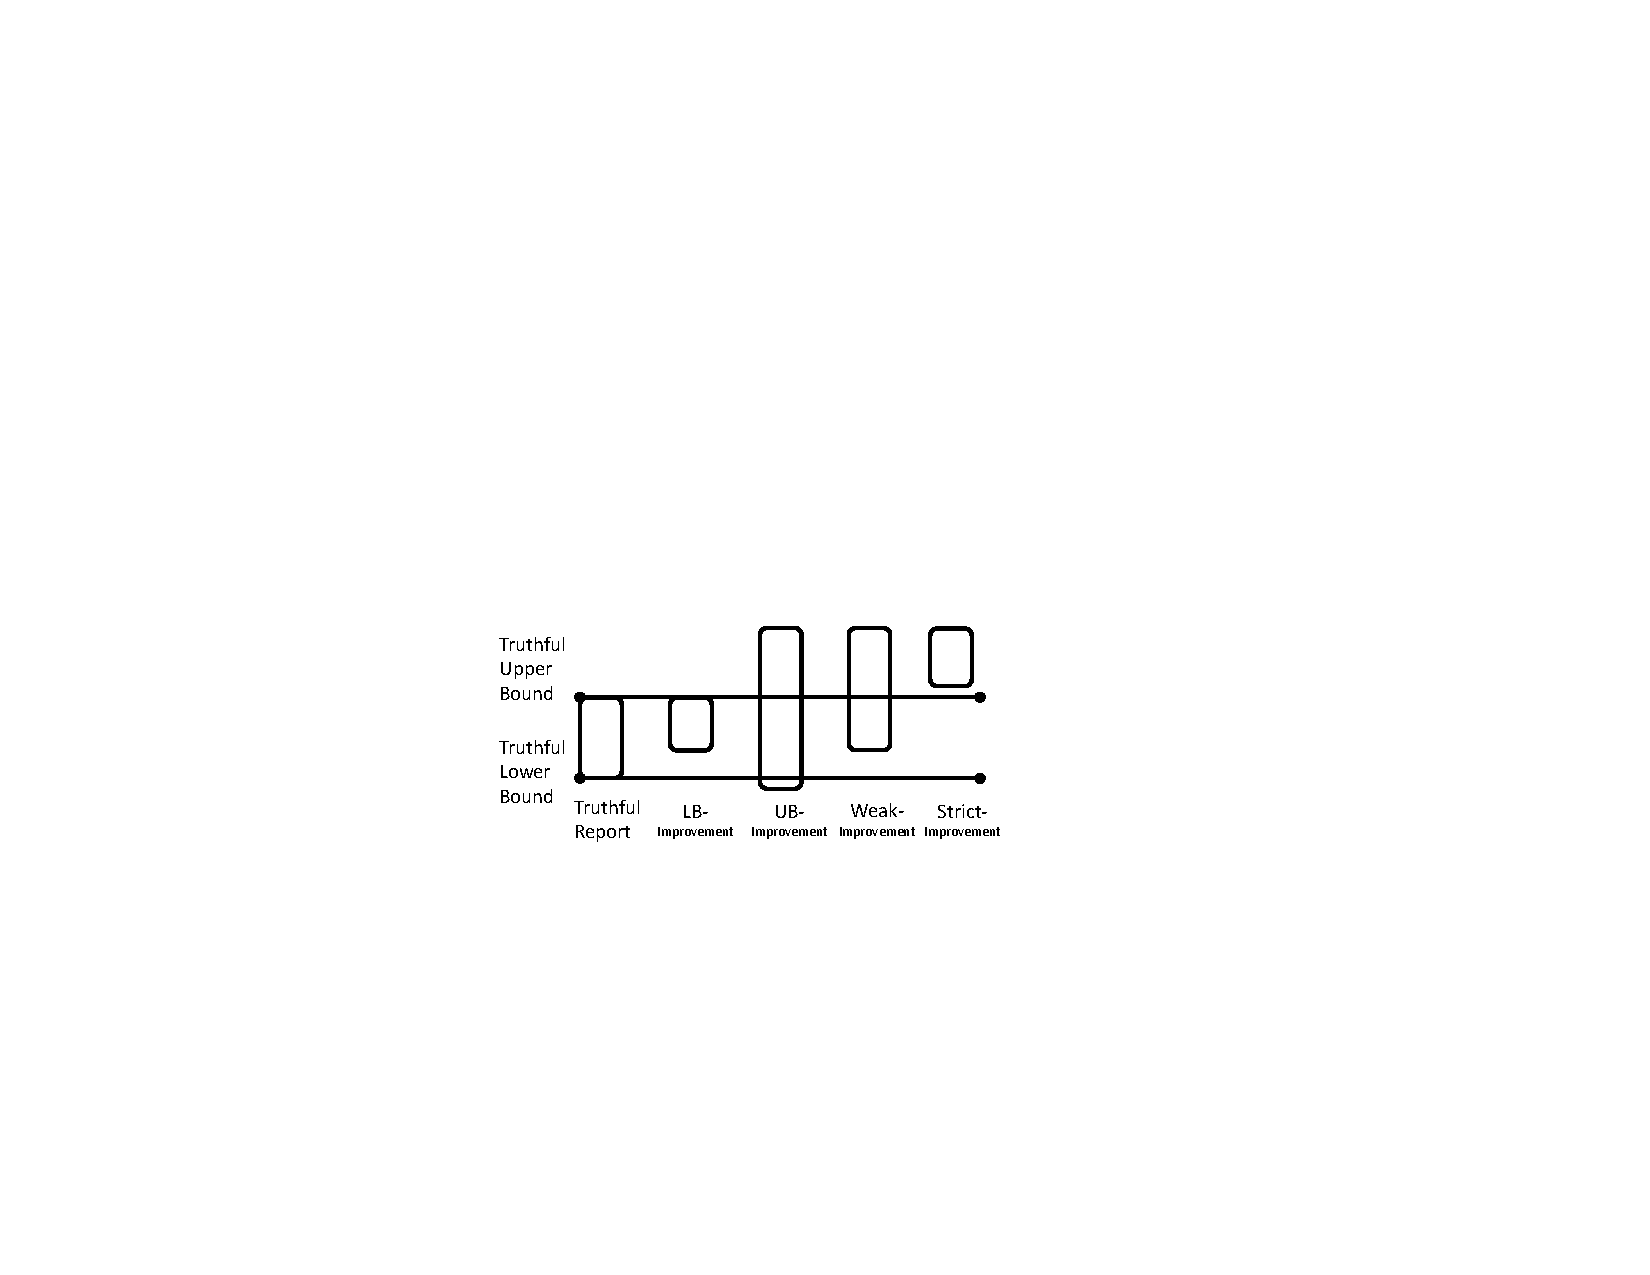
\includegraphics[page=1]{Graphs/manipulation_types.pdf}
     \caption{The possible utility values of the manipulator for each manipulation type.}
 \label{fig:manipulation_types}
\end{figure}

\section{Related Work}


%or by restricting players' preferences and the available coalition formations

%Hedonic games have been widely researched in the literature \cite{aziz2016computational}, and in particular ASHGs \cite{bogomolnaia2002stability}, from strategic point of view with emphasis on stable outcomes such as Nash equilibrium and the core \cite{aziz2011stable, peters2016graphical}. 
%The computational complexity of these problems have been studied in [ref]
%Hedonic games have also been studied from an optimization point of view, where the goal is to find a coalition formation maximizing a global utility function \cite{bachrach2013optimal, bansal2004correlation,charikar2005clustering}. 
There are several studies that developed strategyproof mechanisms for forming coalitions. 
\citeauthor{dimitrov2004enemies} \shortcite{dimitrov2004enemies} discussed ASHGs where agents have both positive and negative edges, and provided a strategyproof algorithm for finding stable outcomes.
\citeauthor{rodriguez2009strategy} \shortcite{rodriguez2009strategy} analyzed strategyproof core stable solutions' properties. They showed that single lapping rules are necessary and sufficient for the existence of a unique core-stable partition.
\citeauthor{aziz2013pareto} \shortcite{aziz2013pareto} showed that the serial dictatorship mechanism is strategyproof with appropriate restrictions over the agents' preferences. 
\citeauthor{flammini2017strategyproof} \shortcite{flammini2017strategyproof} focused on the utilitarian SW in ASHGs and Fractional Hedonic Games, and proposed strategyproof mechanisms at the cost of non-optimal social welfare.
\citeauthor{wright2015mechanism} \shortcite{wright2015mechanism} studied a model of ASHG that is very similar to our model, but instead of restricting the number of coalitions they restricted the size of each coalition. Within their model they proposed a strategyproof mechanism that achieves good and fair experimental performance, despite not having a theoretical guarantee.
%%% A little too wordy for one sentence
%111111111
%All of these works have looked for strategyproof mechanisms, while our approach is to identify and study the situations that need a strategyproof mechanism, and the situations that are robust against manipulations.
All of these works have looked for strategyproof mechanisms, while our approach is to study in which situations a strategyproof mechanism is indeed needed, and in which situations it is not needed since manipulation is impossible.

Our approach is similar to the approach of 
\citeauthor{vallee2014study} \shortcite{vallee2014study}, who studied general hedonic games and Sybil attacks, i.e., manipulations, by adding false agents to the game. \citeauthor{vallee2014study} showed that hedonic games with Nash stability as the solution concept are very robust to Sybil attacks, but when contractual individual stability is the solution concept then every game is manipulable. 
%Noga
Recently, \citeauthor{alonhighschool} \shortcite{alonhighschool} considered the At-least-1 objective, and analyzed whether a group of manipulators can guarantee being in the same coalition in every game. \citeauthor{alonhighschool} showed that such manipulation is almost always impossible.

%In our work we concentrate on $k$-coalitional games. %where exactly $k$ coalitions must be formed.
%%However, the restriction on the number of coalitions has been mostly overlooked.
%\citeauthor{sless2014forming} \shortcite{sless2014forming,sless2018forming} initiated the study of ASHGs where exactly $k$ coalitions must be formed.
%In their model the organizer is able to add connections between agents at some cost, and her goal is to maximize the utilitarian SW.
%\citeauthor{skibski2016k} \shortcite{skibski2016k} studied $k$-coalitional cooperative games under the transferable utility setting, and developed a dedicated extension of the Shapley value for these games.




%utiltarian
%All of the objectives that we study are very common, either in the literature on coalition formation or within the context of graph partitioning. The problem of finding a maximum utilitarian SW has been studied by \citeauthor{aziz2015welfare} \shortcite{aziz2015welfare}.
%When considering the restriction of equal-sized coalitions, the finding of such partition is a known problem called Graph Partitioning \cite{bulucc2016recent}.
%egalitarian
%The egalitarian social welfare had also been studied in the domain of additively separable hedonic games \cite{peters2016graphical, aziz2013computing}.
%at least and Pareto
%The at-least-1 objective had been mostly studied in the context of graph theory \cite{stiebitz1996decomposing, alon2006splitting, bang2016finding}. 
%However, the question about equal-sized coalitions remains unanswered.

\section{Definitions}
\label{sec:defn}
Let $A=\{a_{1},\ldots ,a_{n}\}$ be a finite, non-empty set of agents, and let $G=\tuple{A,E}$ be a graph with no self loops, representing the friendship connections between the agents.
The set of immediate neighbours of $a_{i}$ in $G$ is denoted by $N(a_{i})$.
We also refer to $G$ as the \emph{social network}. A coalition $C\subseteq A$ is a subset of agents; we do not require that agents in a coalition form a connected component in the corresponding social network.
Let $u(a_i,C)$ be the utility that agent $a_i$ would obtain from being in coalition $C$. This value is simply the sum of edges corresponding to the immediate neighbors of $a_i$ that are members of $C$. That is,
$ u(a_{i},C)=|C\cap N(a_{i})|$.


We assume that there is a central organizer that would like to partition the agents into $k$ coalitions in order to satisfy some objective, $obj$.
Let $\Pi_k$ denote the set of partitions of $A$ that contain exactly $k$ non-empty subsets where $0 < k \leq n$. 
We refer to elements of $\Pi_k$ as \emph{coalition structures} (CS), and typically use $P, P', \ldots$ to denote such coalition structures.
We assume that the utility of agent $a$ depends only on the members of her coalition. Therefore, if $P \in \Pi_{k}$, $C\in P$, and $a\in C$, then we use the notation $u(a,P)$ to refer to $u(a,C)$.  
Note that there may be several coalition structures that satisfy a given objective $obj$. We denote this set of coalitions as $O_{obj}(G) \subseteq \Pi_k$ and refer to them as \emph{solutions}. In many cases we  omit the reference to $obj$ when it is clear.

In our setting the social network is formed based on self reports of the agents. That is, each agent $a_i$ is asked by the organizer to list all of her friendship connections. Formally, let $R=\{r_{1},\ldots, r_{n}\}$ be the set of reports, where $r_{i}\subseteq A\setminus\{a_{i}\}$.
In such a scenario there might be a manipulative agent $m$. We begin by assuming that $m$ has full information regarding the social network (we relax this assumption in Section~\ref{sec:limited}) and the objective of the central organizer, $obj$.
Moreover, we assume that $m$ is able to misreport his friendship connections and thus add non-existing edges connecting him to other agents or omit existing edges between him and other agents. %but not do both.
We denote these two types of manipulators by $m^+$ and $m^-$, respectively. We did not consider a manipulator that is capable of both adding and removing edges since it does not add any new results: in all of our objectives only one capability is needed to show susceptibility to manipulation.
Let $G^m=\tuple{A,E^m}$ be the resulting social network known to the organizer after the manipulation $r_m$, and let $N^m(a)$ be the set of immediate neighbours of $a$ in $G^m$.
%% Is this note about directed is still necessary?
Note that if $G$ is directed then we assume that $m$ is able to add or remove only outgoing edges, i.e., add an edge $(m,a_i) \notin E$ or remove an edge $(m,a_i) \in E$. $m$ is not able to add or remove incoming edges, i.e., add an edge $(a_i,m) \notin E$ or remove an edge $(a_i,m) \in E$. That is, $N(a)=N^m(a)$ for every agent $a \neq m$. 
If $G$ is undirected then a manipulation by adding edges is relevant when the organizer adds an edge $(a_i,a_j)$ to $G$ if either $a_i\in r_j$ or $a_j\in r_i$. On the other hand, a manipulation by removing edges is relevant when the organizer adds an edge $(a_i,a_j)$ to $G$ only when both $a_i\in r_j$ and $a_j\in r_i$.
%If $G$ is undirected then a manipulation by adding edges is relevant when the organizer assumes that if an agent $a_i$ report on an edge $(a_i,a_j)$ then both $a_i$ and $a_j$ would like to be in same coalition. On the other hand, a manipulation by removing edges is relevant when the organizer adds an edge $(a_i,a_j)$ to $G$ only when both $a_i$ and $a_j$ report on this edge.
When the context is clear we will sometimes refer to $G^m$ as the manipulation.
 
%Recall that $N(a_i)$ is the set of immediate neighbours of $a_i$ in $G$. Let $N^{m}(m)$ is the set of neighbours the manipulator has after a manipulation. We will denote the new social network as $G^{m}$. (In the case of undirected graphs the manipulation might affect the other agents' neighbours as well.)

%Probably need to add here something small about voting manipulation, what does 'subject to manipulation' means in the literature


Clearly, the goal of the manipulator is a successful manipulation. Indeed, in our setting there are several ways to define what a successful manipulation is, since there may be several coalition structures that satisfy $obj$ in $G$ and in $G^m$, but the utility of $m$ might be different in each such coalition structure. Formally, given a network $G$ and objective $obj$:
%


\begin{definition}
\label{defn:lower_bound_improvement}
A manipulation $r_m$ is a \emph{lower bound improvement} (LB-improvement) for a manipulator $m$ if:
\[
\underset{P\in O_{obj}(G^{m})}{\min}(u(m,P))>\underset{P\in O_{obj}(G)}{\min}(u(m,P)).
\]
%\end{definition}
%

%\begin{definition}
\label{defn:upper_bound_improvement}
A manipulation $r_m$ is an \emph{upper bound improvement} (UB-improvement) for a manipulator $m$ if:
\[
\underset{P\in O_{obj}(G^{m})}{\max}(u(m,P))>\underset{P\in O_{obj}(G)}{\max}(u(m,P)).
\]
\end{definition}
That is, LB-improvement eliminates coalition structures with low utility for the manipulator, while UB-improvement adds coalition structures with higher utility for the manipulator. For example, assume that for an objective $obj$ and a graph $G$ there are two possible CSs. That is, $O_{obj}(G)=\{P_1,P_2\}$. Moreover, assume that $u(m,P_1)=1$ and $u(m,P_2)=2$. If there exists a manipulation $r_m$ where $O_{obj}(G^m)=\{P_2\}$ (or any other $P$ satisfying $u(m,P)=2$) then $G^m$ is a LB-improvement. If there exists a manipulation $r_m$ where $O_{obj}(G^m)=\{P_1,P_3\}$ and $u(m,P_3)=3$ then $G^m$ is an UB-improvement.
LB-improvement can be considered risk aversion of some sort, while UB-improvement suits an optimistic manipulator looking for higher utilities.
%

There is a stronger variant of manipulation which is both LB- and UB-improvement. An even stronger variant is where every coalition structure is strictly better than every possible coalition structure that would have been generated with $m$'s true preferences. Formally:
\begin{definition}
\label{improvement}
A manipulation $r_m$ is a \emph{weak-improvement} for a manipulator $m$ if it is both LB-improvement and UB-improvement for him.
\label{defn:strict_improvement}
A manipulation $r_m$ is a \emph{strict-improvement} for a manipulator $m$ if:
\[
\underset{P\in O_{obj}(G^{m})}{\min}(u(m,P))>\underset{P\in O_{obj}(G)}{\max}(u(m,P)).
\]
\end{definition}

Revisiting our example, a manipulation where $O_{obj}(G^m) = \{P_3\}$ is a strict-improvement. Note that the utility $u(m,P)$ is always calculated over the original graph $G$ with the manipulator's true neighbours.
We refer to the different manipulations: LB, UB, weak, and  strict-improvement, as \emph{manipulation types}.
%When we refer to the utility with respect to $N^m$ we will explicitly write $u^{m}(a,P)$.
Finally, we define the susceptibility and resistance to a manipulation type of a given objective.
\begin{definition}
\label{defn:subject_to_improvement}
An objective $obj$ is \emph{subject to LB-improvement} by manipulator $m$ over (un)directed networks
if there exists a (un)directed social network $G$ and a manipulation $r_m$ such that $r^m$ is a LB-improvement for $m$.
Otherwise, we say that $obj$ is \emph{LB-proof} against $m$.
\end{definition}
The definitions for the other manipulation types are similar.
When an objective is both LB- and UB-proof, we say that it is \emph{strategyproof}. Figure~\ref{fig:manipulation_types} demonstrates the possible utility values of the manipulator for each manipulation type. 



\section{Full Information}
\label{sec:full_info}
We begin our analysis of the objectives and their susceptibility or resistance to the different types of manipulation. % Specifically, in this section almost all of the results (except for Proposition~\ref{Prop:util_full_info}) show resistance to manipulation. 
To show susceptibility to manipulation, we provide figures that depict the scenarios in which manipulation is possible. We use $k=2$ in all of our proofs, but they can easily be extended for any $k$. We use the following notations: In all of the figures the vertex $m$ represents the manipulator. A node is represented by a circle, and a rectangle with a number $X$ represents a clique of $X$ agents. An edge going to (from) a clique represents edges going to (from) all nodes in the clique. An edge going to (from) a clique with a number $X$ represents $X$ edges going to (from) arbitrarily chosen $X$ nodes in the clique. 
If the graph is directed, then an undirected edge $(a,b)$ represents two directed edges, $(a,b)$ and $(b,a)$. If we prove a result regarding an undirected graph and refer to a figure with a directed graph then every directed edge represents an undirected edge. 
Overall, Figure~\ref{fig:add_graphs} provides scenarios for $m^+$ and Figure~\ref{fig:remove_graphs} provides scenarios for $m^-$. Therefore, the dotted edges in Figure~\ref{fig:remove_graphs} are the fake edges that are added by the manipulator, while the dotted edges in Figure~\ref{fig:remove_graphs} are the edges that are removed by the manipulator.

We note that almost all of the susceptibility results in the full information setting (except for Proposition~\ref{Prop:util_full_info}) are derived by the results of susceptibility in the distance 2 setting (see Section~\ref{subsecdist-2}). Therefore, in this section we mostly provide the results regarding resistance to manipulation.

\subsection{Max-Util}
\label{sec:utilirarain}

Maximizing the utilitarian social welfare (Max-Util) is a very common objective in hedonic games \cite{aziz2015welfare}. It was also studied from the perspective of graph theory, since finding a CS (with $k$ coalitions) that maximizes the utilitarian SW is equivalent to finding a minimum $k$-cut \cite{branzei2009coalitional}.  
Utilitarian SW is defined as the sum of the utilities of all agents. Formally, it is $\underset{a\in A}{\sum}u(a,P)$.

%%%%%%%%%%%%%%%%%%%%%%%%%%%%%%%%%%%%%%%%%%%%%%%%%%%%%%
Max-Util is always susceptible to manipulation; in all of the situations that we consider, this objective is subject to strict-improvement. 
Recall that our susceptibility results are derived from the distance 2 setting. However, there is one situation in which the susceptibility to manipulation in the distance 2 setting is not known 
%(see the conjecture in the appendix)
, and thus we show that even in this situation Max-Util is subject to strict-improvement. 
%The objective of maximizing the utilitarian SW is subject to strict-improvement against both $m^+$ and $m^-$. We now show the susceptibility to manipulation by $m^-$, and the susceptibility to manipulation by $m^+$ is implied by Proposition~\ref{prop:util_distance2_add}.



\begin{proposition}
\label{Prop:util_full_info}
Max-Util is subject to strict-improvement by a manipulator $m^-$ over an undirected network.
\end{proposition}
\begin{proof}
Consider the network $G$ as depicted in Figure~\ref{fig:Util_remove_Improve}. Recall that $k=2$. Clearly, the minimum $2$-cut is obtained by cutting the upper clique ($\{a,b,c,d,e,f\}$) from the rest of the network, yielding a minimum $2$-cut of size 3. The manipulator's utility is thus 5. By removing the dotted edges, the minimum $2$-cut is obtained by cutting the lower clique ($\{n,o,p,q,r,s\}$), yielding a minimum cut of size 2. The manipulator's utility is strictly improved from 5 to 6.
\end{proof}

\subsection{Max-Egal}
\label{Sec:egalitarian}
We now consider the objective of maximizing the egalitarian social welfare (Max-Egal), i.e., maximizing the utility of the agent that is worst off. Formally, it is $\underset{a\in A}{\min}(u(a,P))$.
The objective egalitarian social welfare has also been studied in ASHGs \cite{peters2016graphical,aziz2013computing}.
Maximizing the egalitarian SW might result in a decrease in the average utility of the agents  (which is correlated to the utilitarian SW) but it tries to ensure that all of the agents will have some minimum utility. Now, let $Eg(P,G)$ be the egalitarian SW of a coalition structure $P$ in graph $G$. The following theorems show that Max-Egal is resistant to manipulation by adding edges. The intuition is that by adding edges the manipulator is not able to pretend to be the agent with the minimum utility, and he may increase the utility of the other agents by at most $1$. 
\begin{theorem}
\label{thrm:egal_undir_add}
Max-Egal is weak-proof against manipulator $m^+$ over undirected networks.
\end{theorem}
\begin{proof}
%Let $G$ be an undirected network, and $m^+$ a manipulator.
Let 
\[
u_0=\underset{P\in O(G)}{\min}(\{u(m,P)\}),
u_1=\underset{P\in O(G)}{\max}(\{u(m,P)\}).
\]
We will refer to the CS yielding $u_0$ as $P_0$.
Assume by contradiction that Max-Egal is subject to weak-improvement.
That is, there exists a manipulation $r_{m}$ and a CS $P^m\in O(G^{m})$ such that $u(m,P^m) > u_1$. That is, $P^m\notin O(G)$. In addition, 
\begin{equation} \label{ineq:egal_undir}
\forall \  P \in O(G^m), u(m,P) > u_0.
\end{equation}

Since the manipulator can only add edges, it holds that $Eg(P^{m},G^m)\geq Eg(P_0,G)$. Moreover, if $Eg(P^{m},G^m)=Eg(P_0,G)$ then $P_{0}\in O(G^{m})$, which is not possible according to  inequality~\ref{ineq:egal_undir}. Therefore, $Eg(P^{m},G^m)>Eg(P_0,G)$. Since the manipulator is able to add at most one new edge to every agent and $G$ is undirected, then $\forall a \in A \setminus \{m\}$, \[
% = u(a,\P)
u(a,P^{m})  \geq Eg(P^{m},G^m) - 1 \geq Eg(P_0,G).
\]
In addition, $u(m,P^{m})>u_1\geq Eg(P_0,G)$. 
Overall, $\forall a \in A, u(a,P^{m}) \geq Eg(P_0,G)$. That is, $Eg(P^{m},G) \geq Eg(P_0,G)$, and thus $P^m\in O(G)$, which is a contradiction. 
\end{proof}

\begin{theorem}
\label{thrm:egal_dir_add}
Max-Egal is strategyproof against a manipulator $m^+$ over directed networks.
\end{theorem}
\begin{proof}
Let 
\[
u_0=\underset{P\in O(G)}{\min}(\{u(m,P)\}),
u_1=\underset{P\in O(G)}{\max}(\{u(m,P)\}).
\]
We will refer to the CS yielding $u_0$ as $P_0$. Note that for every $P\in O(G)$ it holds that $Eg(P,G) \leq u_0 $.
Assume by contradiction that Max-Egal is subject to UB-improvement.
That is, there exists a manipulation $r_{m}$ and a CS $P^m\in O(G^{m})$ such that $u(m,P^m) > u_1$. That is, $P^m\notin O(G)$.

Since the manipulator can only add edges, it holds that $Eg(P^{m},G^m)\geq Eg(P_0,G)$. Moreover, if $Eg(P^{m},G^m)=Eg(P_0,G)$ then $P_{0}\in O(G^{m})$, which is not possible. Therefore, $Eg(P^{m},G^m)>Eg(P_0,G)$. Recall that in directed networks the utility of the other agents does not change. Therefore $\forall a \in A \setminus \{m\}$, \[
u(a,P^{m})  \geq Eg(P^{m},G^m) > Eg(P_0,G).
\]
In addition, $u(m,P^{m})>u_1\geq Eg(P_0,G)$. 
Overall, $\forall a \in A, u(a,P^{m}) \geq Eg(P_0,G)$. That is, $Eg(P^{m},G) \geq Eg(P_0,G)$, and thus $P^m\in O(G)$, which is a contradiction.


Now, assume by contradiction that Max-Egal is subject to LB-improvement.
That is, there exists a manipulation $r_{m}$ such that
\begin{equation} \label{ineq:egal_dir}
\forall \  P \in O(G^m), u(m,P) > u_0.
\end{equation} That is $P_0\notin O(G^m)$.
Denote an arbitrary CS in $O(G^m)$ as $P^m$. 
It holds that $Eg(P^m,G^m)>Eg(P_0,G^m)$ and $Eg(P_0,G)\geq E(P^m,G)$.

Again, in directed networks the utility of the other agents does not change. Therefore, if after the manipulation $Eg(P^m,G^m)>Eg(P^m,G)$, it can only change by the utility of $m$. But $u(a,P^m)>u(a,P)$, hence even before the manipulation $Eg(P^m,G^m)>Eg(P^m,G)$, in contradiction.
\end{proof}


\subsection{At-least-1}
\label{sec:least1}
In the At-least-1 objective the organizer is only interested in ensuring that every agent will have a utility of at least $1$. This objective is very general, and it may result in many possible CSs. It has mostly been studied in the context of graph theory \cite{stiebitz1996decomposing,alon2006splitting,bang2016finding}.

Note that there are some instances where there is no CS that guarantees a utility of at least $1$ to every agent. We call such an instance \textit{infeasible}, and we then write $O(G) = \emptyset$. In infeasible instances we assume that the utility of all of the agents is $0$.
%organizer might choose any CS. Therefore, the lower and upper bounds for a manipulator in an infeasible instance are $0$ and $N(m)$, respectively.
%Trivially, due to this assumption, the At-least-1 objective is subject to UB-improvement against a manipulator $m^-$: consider any feasible instance in which the utility of the manipulator $m$ is less than $N(m)$. The manipulator can remove all of his edges, making the instance infeasible, and thus improving his upper bound. 
%Indeed, such manipulations also set the lower bound to $0$. Similarly, the At-least-1 objective is subject LB-improvement against a manipulator $m^+$ over undirected networks: consider an instance in which the manipulator is part of a clique, and there is one additional agent, $x$, with no edges at all. Clearly, this is an infeasible instance, but the manipulator can add an edge to $x$, making the instance feasible, and thus improving his lower bound. Since these are trivial manipulations, for the rest of the paper we restrict our analysis to feasible instances, and we also assume that the manipulator is not allowed to make an instance infeasible.
%
We show that, in contrast to the previous objectives, At-least-1 is less susceptible to manipulations. Specifically, we show that an UB-improvement is almost always impossible, and LB-improvement is impossible by adding directed edges. The intuition is that adding edges is beneficial only if the network is undirected and the new edges transform an infeasible instance into a feasible instance, and by removing edges the manipulator is not able to introduce new solutions.
%

\begin{theorem}
\label{thrm:least1_add_dir}
At-least-1 is strategyproof against manipulator $m^+$ over directed networks.
\end{theorem}
\begin{proof}
%Let $G$ be a network and $m^+$ a manipulator. 
Let $u_1=\underset{P\in O(G)}{\max}(\{u(m,P)\})$, and recall that if $O(G) = \emptyset$ then $u_1=0$.
Assume by contradiction that the At-least-1 objective is subject to UB-improvement.
That is, there exists a manipulation $r_{m}$ and a coalition structure $P^m\in O(G^{m})$ such that $u(m,P^m) > u_1$. That is $P^m\notin O(G)$, and $\forall a \in A, |N^m(a)| \geq 1$.
Since $u_1 \geq 0$ then $u(m,P^m) \geq 1$. 
In addition, recall that in a directed network, $\forall a \in A \setminus \{m\}, N(a)=N^m(a)$, thus $\forall a \in A \setminus \{m\}, u(a,P^m) \geq 1$.
Overall, $\forall a \in A, u(a,P^m) \geq 1$ and thus $P^m \in O(G)$, which is a contradiction.

%u(a,P^m,G^m)=u(a,P^m)

% If $O(G)$ is empty, there can not be a LB-improvement as that would imply an UB-improvement as well.

Regarding  LB-improvement, since the manipulator is only able to add edges then $O(G) \subseteq O(G^m)$. Therefore, no LB-improvement is possible if $O(G) \neq \emptyset$. 
If $O(G) = \emptyset$, then $u_1=0$. Now, assume by contradiction that the At-least-1 objective is subject to LB-improvement. That is, there exists a manipulation $r_{m}$ for which $\underset{P\in O(G^m)}{\min}(\{u(m,P)\})$ is at least $1$. Since $u_1=0$ that would imply an UB-improvement as well, which is impossible (as shown above).
\end{proof}

\begin{theorem}
\label{thrm:least1_remove}
At-least-1 is UB-proof against manipulator $m^-$ over directed and undirected networks.
\end{theorem}
\begin{proof}
Since $m$ is only able to remove edges then for every manipulation $r_m$ it holds that $O(G^m) \subseteq O(G)$. Therefore, $\underset{P\in O(G)}{\max}(\{u(m,P)\})\geq \underset{P\in O(G^m)}{\max}(\{u(m,P)\}) $ and no UB-improvement is possible. 
\end{proof}





\section{Limited Information}
\label{sec:limited}
We now focus on more realistic settings, in which the manipulator is not familiar with the full structure of the network. Instead, we assume that the manipulator is either familiar only with his immediate neighbours in the network, or he may also be familiar with the neighbours of his immediate neighbours. Within this setting we need to revise our definitions of successful manipulations. Specifically, since the manipulator is familiar only with a partial network, we define suitable safe manipulations. Informally, a safe manipulation is a manipulation in which the manipulator is not worse off in all of the possible completions of the partial network, and there exists at least one completion of the partial network in which the manipulator is better off.  

Formally, let $A_0 = \{m\}$.
Let $G_1=(A,E_1)$ be a graph, $E_1 \subseteq E$, where $(u,v) \in E_1$ if either $u$ or $v$ belongs to $A_0$.
Similarly, let $A_1 = \{u : (u,v) \in E_1 \lor  (v,u) \in E_1\}$.
Let $G_2=(A,E_2)$ be a graph, $E_2 \subseteq E$, where $(u,v) \in E_2$ if either $u$ or $v$ belongs to $A_1$.
%
%
%Formally, let $dis(a,a')$ be the length of the shortest path in $G$ between two vertices $a,a' \in A$. We call $dis(a,a')$ the distance between $a$ and $a'$.
%Let $G_d=(A,E_d)$ be a graph, $G_d \subseteq G$, and $E_d \subset E$, where $(a,a') \in E_d$ if $dis(a,m) \le d$ or $dis(a',m) \le d$.
%
%contains only edges going to or from neighbours of distance at most $d-1$ from $m$.
Given $d \in \{1,2\}$, a \emph{possible network} $\overline{G_d}$ of $G_d$ is a network $\overline{G_d}=(A,\overline{E_d})$ where $\overline{E_d} = E_d \cup E'$ such that if $(u,v)\in E'$ then neither $u$ and $v$ belong to $A_{d-1}$.
We assume that the manipulator is familiar with $G_d$ and the objective $obj$.
We denote the settings in which the manipulator is familiar with $G_1$ ($G_2$) by \emph{distance 1} (\emph{distance 2}). 
Indeed, since the manipulator is always familiar with his immediate neighbours he can still add or remove edges as in the full information setting. However, since the manipulator is only familiar with $G_d$ he needs to consider the effect of his manipulation  on every possible network $\overline{G_d}$. Given $\overline{G_d}$ and a manipulation $r_m$, let $\overline{G_d}^m$ be the possible network after the manipulation $r_m$.
We can now revise our definitions of successful manipulations.
Given a partial network $G_d$ and an objective $obj$:
\begin{definition}
A manipulation $r_m$ is a \emph{d-safe lower bound improvement} for a manipulator $m$ if for all possible networks $\overline{G_d}$ of $G_d$ it holds that
\[
\underset{P\in O_{obj}(\overline{G_d}^m)}{\min}(u(m,P))\geq\underset{P\in O_{obj}(\overline{G_d})}{\min}(u(m,P)).
\]
and for at least one possible network $\overline{G_d}$, $r_m$ is a LB-improvement.

%If for all possible networks $\overline{G}$, $r_m$ is not a LB-improvement we say the manipulation is \emph{not profitable}, and if for at least one possible network $\overline{G}$ the manipulation lowers the LB of $m$ we say it is \emph{LB-unsafe}.
% \end{definition}


% \begin{definition}
% A manipulation $r_m$ is a \emph{d-safe weak-improvement} (\emph{d-safe strict-improvement}) for a manipulator $m$ if for all possible networks $\overline{G_d}$ of $G_d$ it holds that
% \[
% \underset{P\in O_{obj}(\overline{G_d}^{m})}{\min}(u(m,P))\geq\underset{P\in O_{obj}(\overline{G_d})}{\min}(u(m,P)).
% \]
% \[
% \underset{P\in O_{obj}(\overline{G_d}^{m})}{\max}(u(m,P))\geq\underset{P\in O_{obj}(\overline{G_d})}{\max}(u(m,P)).
% \]
% and for at least one possible network $\overline{G_d}$, $r_m$ is a weak-improvement (strict-improvement).
%\end{definition}


%\begin{definition}
An objective is \emph{subject to d-safe LB-improvement} by manipulator $m$ over (un)directed networks if there exists a (un)directed partial network $G_d$ and a manipulation $r_m$ such that $r_m$ is a d-safe LB-improvement for $m$. Otherwise we say that \emph{obj} is \emph{d-safe LB-proof} against $m$.
\end{definition}
\noindent
The definitions for the other manipulation types are similar. Note that susceptibility to d-safe manipulation implies susceptibility to d'-safe manipulation for any $d'>d$, as well as to the full information case. Similarly, resistance to manipulation in the full information setting implies resistance to manipulation in the limited information setting.
%of \emph{d-safe UB improvement, d-safe improvement, subject to d-safe LB-improvement, subject to d-safe improvement, subject to d-safe strict improvement, d-safe LB-improvement, d-safe improvement proof} and \emph{d-safe strict improvement proof} 
%Due to space constraints, the proofs of most of the theorems in this section are provided in the full version of this paper \cite{fullversion}. However, we  provide references to the figures that depict the safe manipulations.
\begin{figure*}[t]
    \centering
    \centering  
        \begin{subfigure}{0.1\textwidth}
            \centering
            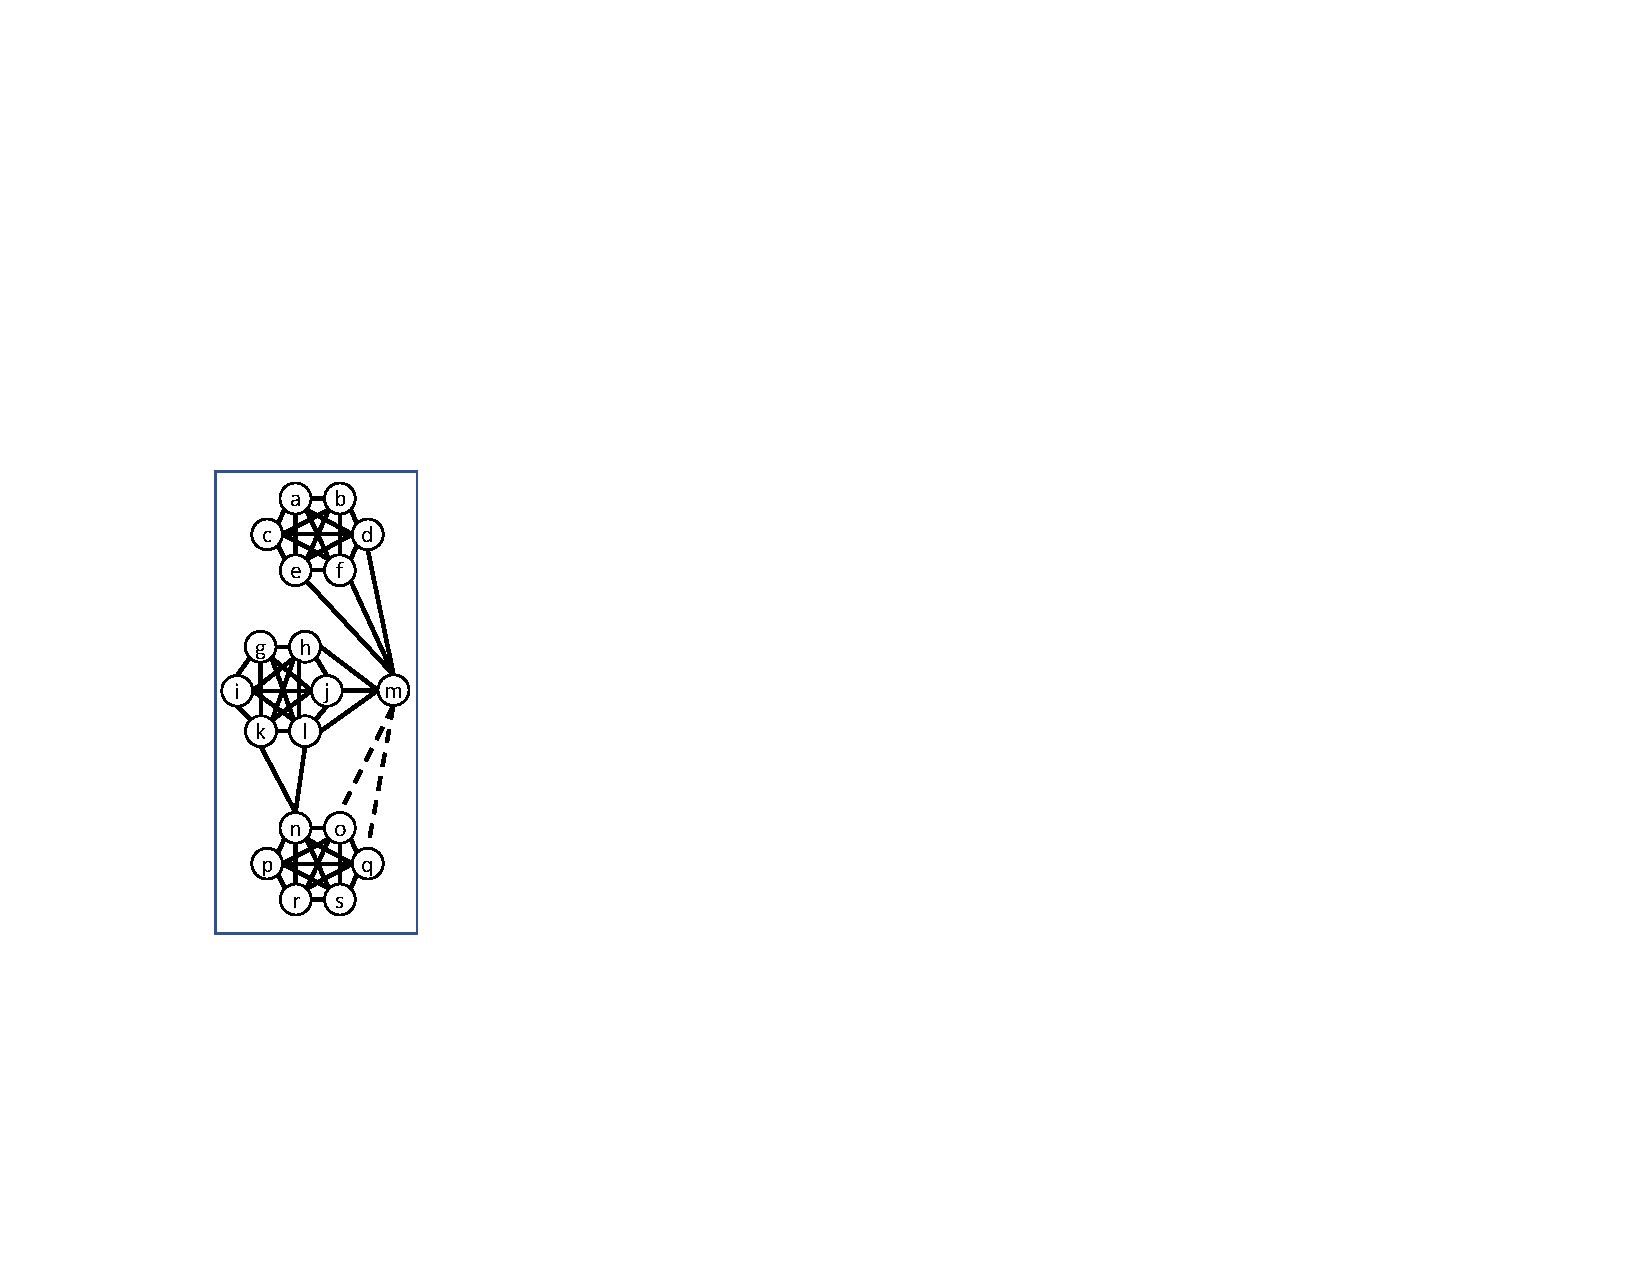
\includegraphics[page=1,width=\textwidth]{Graphs/graphs.pdf}
            \caption{\\U/S}
            \label{fig:Util_remove_Improve}
        \end{subfigure}    
        \hfill
        \begin{subfigure}{0.1\textwidth}
            \centering
            \includegraphics[page=47,width=\textwidth]{Graphs/graphs.pdf}
            \caption{\\U/S}
            \label{fig:Util_dir_remove}
        \end{subfigure}
        \hfill
        \begin{subfigure}{0.1\textwidth}
        \centering
            \includegraphics[page=6,width=\textwidth]{Graphs/graphs.pdf}
            \caption{\\U/LB}
            \label{fig:Util_remove_LB}
        \end{subfigure}    
        \hfill
        \begin{subfigure}{0.1\textwidth}
        \centering
            \includegraphics[page=9,width=\textwidth]{Graphs/graphs.pdf}
            \caption{\\U/UB}
            \label{fig:Util_remove_UB}
        \end{subfigure}
        \hfill
        \begin{subfigure}{0.1\textwidth}
        \centering
            \includegraphics[page=19,width=\textwidth]{Graphs/graphs.pdf}
            \caption{\\E/S}
            \label{fig:Egal_directed_remove}
        \end{subfigure}
        \hfill
        \begin{subfigure}{0.1\textwidth}
            \centering
            \includegraphics[page=17,width=\textwidth]{Graphs/graphs.pdf}
            \caption{\\E/S}
            \label{fig:Egal_undirected_remove}
        \end{subfigure}
        \hfill
        \begin{subfigure}{0.1\textwidth}   \centering
            \includegraphics[page=31,width=\textwidth]{Graphs/graphs.pdf}
            \caption{\\1/LB}
            \label{fig:least1_remove}
        \end{subfigure}
    
    \caption{Figures for the proofs of manipulations by $m^-$. Key:U=Max-Util, E=Max-Egal, 1=At-least-1, S=strict-improvement, UB=UB-improvement, LB=LB-improvement}
    %graphs showing manipulation of different objectives by adding edges. Dotted edges are added by the manipulator.
    \label{fig:remove_graphs}
\end{figure*}

\begin{figure}[t]
    \centering  
        \begin{subfigure}{0.09\textwidth}
            \centering
            \includegraphics[page=3,width=\textwidth]{Graphs/graphs.pdf}
            \caption{\\U/S}
            \label{fig:Util_add}
        \end{subfigure}
        \hfill
        \begin{subfigure}{0.09\textwidth}
            \centering
            \includegraphics[page=12,width=\textwidth]{Graphs/graphs.pdf}
            \caption{\\E/LB}
            \label{fig:Egal_undirected_add_LB}
        \end{subfigure}
        \hfill
        \begin{subfigure}{0.09\textwidth}
            \centering
            \includegraphics[page=15,width=\textwidth]{Graphs/graphs.pdf}
            \caption{\\E/UB}
            \label{fig:Egal_undirected_add_UB}
        \end{subfigure}
        \hfill
        \begin{subfigure}{0.09\textwidth}
            \centering
            \includegraphics[page=49,width=\textwidth]{Graphs/graphs.pdf}
            \caption{\\1/S}
            \label{fig:Least1_undirected_add}
        \end{subfigure}
    
    
    \caption{Figures for the proofs of manipulations by $m^+$. Key:U=Max-Util, E=Max-Egal, 1=At-least-1, S=strict-improvement, UB=UB-improvement, LB=LB-improvement}
    %graphs showing manipulation of different objectives by adding edges. Dotted edges are added by the manipulator.
    \label{fig:add_graphs}
\end{figure}

{\small
\begin{table}[t]
\ra{1}
\begin{tabular}{@{}llllr@{}}\toprule 
$Objective$ & $Manipulator$ & $Network$ &  $Type$ & $Fig$\\\midrule
Max-Util & Add & Both & Strict & \ref{fig:Util_add}\\
Max-Util & Remove & Directed & Strict & \ref{fig:Util_dir_remove}\\
Max-Util & Remove & Undirected & LB & \ref{fig:Util_remove_LB}\\
Max-Util & Remove & Undirected & UB & \ref{fig:Util_remove_UB}\\
Max-Egal & Add & Undirected & LB & \ref{fig:Egal_undirected_add_LB}\\
Max-Egal & Add & Undirected & UB & \ref{fig:Egal_undirected_add_UB}\\
Max-Egal & Remove & Directed & Strict & \ref{fig:Egal_directed_remove}\\
Max-Egal & Remove & Unirected & Strict & \ref{fig:Egal_undirected_remove}\\
At-Least-1 & Add & Undirected & Strict & \ref{fig:Least1_undirected_add}\\
At-Least-1 & Remove & Both & LB & \ref{fig:least1_remove}\\
\bottomrule
\end{tabular}
\caption{Summary of susceptibility results for distance 2.
Key: LB/UB/Strict = the objective is subject to LB/UB/Strict-improvement.
}
\label{tbl:distnce2_summary}
\end{table}
%discussions
}
\subsection{Distance 1}
\label{sec:distance1}
We analyze the three objectives and their susceptibility to safe manipulations in the setting of distance 1. Remarkably, even in this setting there are situations where a safe manipulation exists (Proposition~\ref{prop:distance1}). 
However, Theorem~\ref{thm:all_distance1} shows that for most situations safe manipulation is impossible. The proof is based on extensive enumeration of networks, where we show that either no manipulation exists or there exists only an unsafe manipulation.

\begin{proposition}
\label{prop:distance1}
Max-Egal against manipulator $m^-$ over directed networks and At-Least-1 against $m^+$ over undirected networks are subject to 1-safe UB-improvement.
\end{proposition}

\begin{proof}
Figure~\ref{fig:distance1_egal_ub_any} provides proof for Max-Egal.
Clearly, At-Least-1 is subject to UB-improvement by simply adding any edge, as it can turn an infeasible instance into a feasible instance.
\end{proof}

\begin{theorem}
\label{thm:all_distance1}
All three objectives are 1-safe strategyproof except for the cases in Proposition~\ref{prop:distance1}.

\end{theorem}

\begin{proof}[Proof (partial)]
\textbf{Max-Util}. 
We show that Max-Util is 1-safe strategyproof against manipulators $m^-$ and $m^+$ over undirected networks. We start with $m^-$;
If $0<|N(m)|<n-1$, Figures \ref{fig:distance1_util_unsafe_remove_LB} and \ref{fig:distance1_util_unsafe_remove_UB} show that removing any edge is UB-unsafe and LB-unsafe, respectively.
Clearly, the graphs in these Figures can be extended to any number of agents and any number of neighbours of the manipulator. For example, to extend figure \ref{fig:distance1_util_unsafe_remove_UB} to arbitrary numbers of agents and neighbours do as following: Connect all of the manipulator's neighbours but one to form a clique ($a,b,c$ in the example). Let the other agents form a clique of their own ($e,f,g,h$ in the example). Lastly connect the manipulator's neighbour which is not in the clique ($d$ in the example) to the other clique with only one edge. This way removing an edge is UB-unsafe.

If $|N(m)|=n-1$,
%
% UB
% 1. remove 1 edge - not ub manipulation
% 2. remove 2 edges - ub-unsafe, since it may be a complete graph
% LB
% 1. remove 1 edge - lb-unsafe (complete graph with one missing)
we first show that Max-Util is 1-safe UB-proof.
If the manipulator removes only 1 edge then he cannot improve his upper bound at all.
%(Detailed explanation is given in the appendix)
If the possible network was a complete graph with $n$ nodes, then removing two edges or more is UB-unsafe.
To see that Max-Util is 1-safe LB-proof, look at a complete graph where one edge is missing (an edge not connected to $m$). Removing any edge in that case can only lower the manipulator's LB.
%

Continuing with $m^+$, if $0<|N(m)|<n-1$ then Figures \ref{fig:distance1_util_unsafe_add_LB},\ref{fig:distance1_util_unsafe_add_UB} show that adding any edge is LB- and UB-unsafe respectively.
Again, these examples can be extended to fit any number of agents and any number of neighbours the manipulator has.
If $|N(m)|=n-1$, the manipulator cannot add edges.

\textbf{At-Least-1}.
For At-Least-1, we prove that the objective is 1-safe LB-proof against manipulator $m^-$. Clearly, At-Least-1 is 1-safe LB-proof over undirected networks, since removing any edge might lead to an infeasible instance. For example, if the manipulator removes an edge from a neighbour that has a degree of one, this neighbour will have a degree of zero in every coalition structure, resulting in an infeasible instance.

Over directed networks, there are two possible cases. If there is an agent $a$ such that $(a,m), (m,a) \in E$, then it is possible that the only feasible coalition structure $P$ is where there is a coalition $C \in P$, $C = \{m,a\}$. Therefore, removing the edge $(m,a)$ results in an infeasible instance. If there is an agent $a$ such that $(m,a) \in E$ but $(a,m) \notin E$, then it is possible that there is an agent $a'$ such that $(a,a'), (a',m) \in E$ and the only feasible coalition structure $p$ is where there is a coalition  $C \in P$, $C = \{m,a,a'\}$. Therefore, removing the edge $(m,a)$ results in an infeasible instance.

Due to space constraints, the complete proof, including the setting of Max-Egal, is provided in the full version of this paper~\cite{waxman2021manipulation}. 
\end{proof}

\subsubsection{Distance 2}
\label{subsecdist-2}
Unlike in the distance 1 setting, the results for the distance 2 setting are almost the same as the results in the full information setting. Indeed, all of the resistance results are derived by the resistance results in the full information setting. Therefore, in this section we provide only  susceptibility results summarized in Table~\ref{tbl:distnce2_summary} where each entry represents a situation, what type of manipulation it is subject to, and a reference to a figure providing a proof. Note that the figures showcase a possible network. The partial network known to the manipulator can easily be derived from them. %Because of space constraints the proofs these manipulations are safe are given in the appendix.
% As for resistance proofs, the proofs hold for any $k$..
%\subsubsection{Max-Util}
Overall, we show that, surprisingly, all of the results for the full information setting hold for the distance 2 setting, except for one case: when maximizing the utilitarian SW, with a $m^-$ manipulator over undirected networks. In this case, Proposition~\ref{Prop:util_full_info} shows that the objective is subject to strict-improvement with full information while Figures~\ref{fig:Util_remove_LB} and \ref{fig:Util_remove_UB} only show that it is subject to 2-safe LB- and UB-improvement in the distance 2 setting. Indeed, we believe that the objective is 2-safe weak-proof.
%\begin{conjecture}
%\label{conj:util}
%Max-Util is 2-safe weak-proof against manipulator $m^-$ over undirected networks.
%\end{conjecture}




\begin{figure}[t]
    \centering
        \begin{subfigure}{0.09\textwidth}
            \centering
            \includegraphics[page=2,width=\textwidth]{Graphs/Distance_1_paper.pdf}
            \caption{R/U/LB}
            \label{fig:distance1_util_unsafe_remove_LB}
        \end{subfigure}
        \hfill
        \begin{subfigure}{0.09\textwidth}
            \centering
            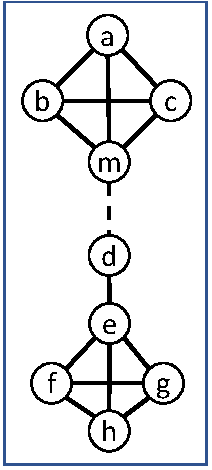
\includegraphics[page=1,width=\textwidth]{Graphs/Distance_1_paper.pdf}
            \caption{R/U/UB}
            \label{fig:distance1_util_unsafe_remove_UB}
        \end{subfigure}
                \hfill
                \begin{subfigure}{0.09\textwidth}
            \centering
            \includegraphics[page=4,width=\textwidth]{Graphs/Distance_1_paper.pdf}
            \caption{A/U/LB}
            \label{fig:distance1_util_unsafe_add_LB}
        \end{subfigure}
                \hfill
                \begin{subfigure}{0.09\textwidth}
            \centering
            \includegraphics[page=3,width=\textwidth]{Graphs/Distance_1_paper.pdf}
            \caption{A/U/UB}
            \label{fig:distance1_util_unsafe_add_UB}
        \end{subfigure}
                \hfill
                \begin{subfigure}{0.09\textwidth}
            \centering
            \includegraphics[page=5,width=\textwidth]{Graphs/Distance_1_paper.pdf}
            \caption{R/E/UB}
            \label{fig:distance1_egal_ub_any}
        \end{subfigure}
    
    \caption{Figures for the proofs of safe and unsafe manipulations, distance 1. Key:U=Max-Util, E=Max-Egal, UB=UB-improvement, LB=LB-improvement, R=Remove, A=Add}
    %graphs showing manipulation of different objectives by adding edges. Dotted edges are added by the manipulator.
    \label{fig:distance1_graphs}
\end{figure}


\section{Discussion}
In this section we discuss our results. We explain the different phenomena that we observe when comparing the results for the different settings.
Our results indicate that manipulations over undirected networks are easier than manipulations over directed networks. This is due to the fact that in directed networks the manipulator can only influence his own utility. In undirected networks the manipulator can actually influence the utility of his neighbours, and this additional power enables the manipulation in additional situations.
We can also observe that Max-Util is the easiest objective to manipulate when compared with Max-Egal and At-least-1. Indeed, Max-Util is inherently different from the other two objectives: when maximizing the utilitarian SW, the organizer is interested in the average utility, thus the organizer always takes into account the utility of the manipulator. In contrast, in the other two objectives the organizer is interested in the utility of the weakest agents, thus the organizer may not take into account the utility of the manipulator (e.g., if the manipulator already has a utility of $5$ in the At-least-1 objective). 
This characteristic of Max-Egal and At-least-1 objectives can also explain why it is easier to manipulate these objectives by removing edges rather than by adding edges: by removing edges the manipulator can pretend to be the weakest agent, affecting the organizer's choice of the coalition structure. Following this observation, we would expect that manipulating the At-least-1 objective will be harder than manipulating the Max-Egal objective: in At-least-1 the organizer is interested only in ensuring a minimum utility of $1$ while in Max-Egal the organizer is also interested in maximizing the minimal utility. However, it turns out that At-least-1 can be manipulated by turning an infeasible instance into a feasible instance, thus there are situations in which At-least-1 is subject to strict-improvement while Max-Egal is weak-proof.
Finally, we note that there is a significant difference between results for the settings of distance 1 and distance 2. In the setting of distance 1, the manipulator has very limited knowledge of the network. Therefore, it is hard for the manipulator to estimate the full effect of adding or removing edges, thus finding that a safe manipulation is impossible in most of the situations. Surprisingly, even though the manipulator is not familiar with the full structure of the network in the setting of distance 2, the additional information in this setting is sufficient for finding safe manipulations in many situations.
%This could be explained by that knowing which neighbours of the manipulator are in a good position and which are not, the manipulator can make good assessments regarding which neighbour it is safe to disconnect from, or which non-neighbours it is worthwhile to connect to.

% distance 1, in almost all situations it is not possible to manipulate. This is not surprising, as the manipulator has almost no knowledge about the graph. However, in distance 2 there are many situations where the amount of knowledge given to the manipulator is sufficient for manipulation, to the level that in all situations but one, if an objective is subjec to manipulation in full information, it is also subject to manipulation in distance 2.


% Distance 1 - almost no knowledge, cannot safely manipulate.
% Distance 2 is enough surprisingly.
%why distance 1 is so weak? because many changes may affect you. With distance 2 there are instances where you have some info

\section{Conclusions and Future Work}
We have studied manipulation in the setting of a central organizer that would like to partition a social network into $k$ coalitions. 
The organizer has a certain objective she would like to satisfy or maximize, whereas there is a manipulator that would like to maximize his utility, i.e., the number of friends within his coalition.
We have distinguished between a manipulator who has full information regarding the structure of the social network, and a manipulator that is only familiar with the edges in close proximity to him. 
%We have shown that these two definitions collide almost always with regards to manipulation capability.
An important future research direction to explore is the complexity of finding a manipulation, given a specific objective. We would also like to extend our analysis to the setting with weighted social networks, or social networks with negative edges.
%New objectives where distance 1 is sufficient for manipulation?
%Find the minimum distance required for manipulation? (only 1 relevant case in our paper where we don't know, but for new objectives
%Characterize objectives that are subject/resistace to manipulation types.
%Find objective where add+remove gets new powers



%When she knows the partial network at distance 2 all the results but one collide with the ones in full information, showing that if there exists an instance in full information which is susceptible to manipulation, almost always there exists an instance in limited information which is also susceptible to manipulation. 

\section*{Acknowledgements}
This work has been supported in part by the Israel Science
Foundation under grant 1958/20, the Ministry of Science, Technology \& Space, Israel and the EU project TAILOR under
Grant 992215.

\bibliographystyle{named}
\bibliography{bib}








\end{document}